\par Now, that the topic of the thesis was introduced and the question of the research was stated, there are necessary preliminaries that need to be mentioned and explained, in order have a better understanding fpr the following chapters. \\ Thus, we will clarify the basics of the \textit{microgrids} and in particular the \textit{(prosumer-based) DC microgrids} (\ref{sec:dcmicrogrids}), \textit{power network modeling} (\ref{sec:power_network})and the \textit{iterative learning control} method (\ref{sec:ilc})
 
\section{Basics of prosumer-based DC microgrids}
\label{sec:dcmicrogrids}
\par In this section we are going to introduce the (prosumer-based DC) microgrid concept. Firstly, in order to understand the functionality of the microgrids and especially the DC microgrids, which are going to be introduced later, we should discuss, what \textit{Distributed generation} is.
\subsection{Distributed generation}
\label{subsec:der}
Distributed generation is the electrical generation and storage performed by a variety of small, grid-connected or distribution system-connected devices referred to as distributed energy resources (\textit{DER}), as defined in \cite{dg_wiki}. DER systems typically use renewable energy sources such as e.g. biogas, fuel cells, solar power or wind power \cite{dg_wiki}. Different from a transmission network, distributed generation basically generates electricity close to the consumer, which means that the efficiency of the current generation plant usually only covers the energy demand of current consumers that are directly next or in the closer environment.
\\Another difference between distributed and the central generation, as described in \cite{epa_dg} is, that the distributed resources work with low voltages, with the central generators are provided through the higher voltages. Therefore, distributed generation can reduce electricity losses along transmission and distribution lines when connected to the electric utility’s lower voltage distribution lines \cite{epa_dg}. It can also provide lower-cost electricity and higher power reliability and security with fewer environmental consequences such in the common power generators. 
\\Distributed generation can be a single structure, such as a home or a place of residence, or it may be part of a \textit{microgrid}, such as a large college campus or a industrial plant \cite{dg_wiki}. \par Since the operation area of a microgrid is now clarified, we will introduce in the next subsection with the microgrid and in particular the DC microgrid.
\subsection{ Microgrids}
\label{subsec:microgr}
\begin{figure}[h]
\begin{center}
    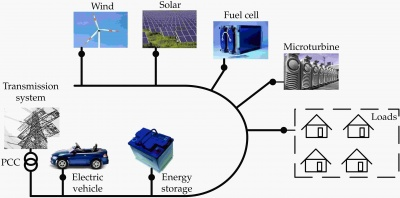
\includegraphics[scale=0.8]{pictures/microgrid_concept.jpg}
    \caption{The microgrid concept}
    \label{figure_microgrid_concept}
\end{center}
\end{figure}
In this scope we are going to use the definition of a microgrid as in \cite{Hatzi}.
\begin{definition} from \cite{Hatzi} \\
"Microgrids comprise LV distribution systems with [...] DER (microturbines, fuel cells, PV, etc.) together with storage devices (flywheels, energy capacitors and
batteries) and flexible loads. Such systems can be operated in a non-autonomous way, if
interconnected to the grid, or in an autonomous way, if disconnected from the main grid. The
operation of microsources in the network can provide distinct benefits to the overall system
performance, if managed and coordinated efficiently."
\end{definition}
By this definition we understand that a microgrid consists of a limited number of generation units, storage units and demand resources, all together located in a local distribution grid, as sketched in \ref{figure_microgrid_concept} \cite{microgrid_concept}. Microgrids do not always have a synchronous connection to the main generation net which means that the tasks that are necessary for a constant and safe operation need to be provided, in cases of emergency \cite{concept}. They should though have the option of a synchronous connection to the main generation network. Such systems arise from the geographical circumstances that make a connection to the main network costly and almost impossible. Microgrids on the other hand serve to an increased security of supply, should a collaps of the main network occur \cite{concept}.\\ An introduction on the alternating and direct current microgrids is given in the next section. Since the main focus of this thesis is on the direct current type of microgrids, the alternating current will be only mentioned summarized.  
\subsection{Direct current versus alternating current microgrids}
\label{subsec:acdc}
\par Electric charge in \textit{alternating current} (AC) changes direction periodically and is characterized by an amplitude and a frequency. The electric charge in \textit{direct current} (DC) on the other hand only flows in one direction and remains constant the whole time. Back in time, DC could not be easily converted to high voltages due to the high transformation losses. Therefore, AC is the preferred type of current for power networks and used until today \cite{mikieus}, but with the development of the DC-based power electronics for generating as well as load that allow efficient voltage transformation, DC is on the rise again and more often used in microgrids.
\\ In \cite{versus}, Table 4 in [25, p.399] a comparison between AC and DC microgrids is given. Since the line losses (the power that is lost in a conductor during transmission and distribution phase, as in \cite{lineloss}) in AC distribution are high, it leads to less efficiency and less power transmission. In DC distribution the power transmission is more efficient due to a lower line loss, no reactance in the line and a low line resistance itself. DC distribution does not obviously require frequency monitoring, since the frequency of DC is constantly zero, has no electromagnetic interference, like AC distribution does and is easier when it comes to the analysis, since only real numbers are involved. \\
Hence, DC distribution is chosen in this work due to higher efficiency and lower line losses. Finally, prosumer-based DC microgrid is defined in the next section.
\subsection{Prosumer-based (DC) microgrids}
\label{subsec:prosumer}
\par In \ref{subsec:der}, it is mentioned that " [...] distributed generation basically generates electricity close to the consumer [...]". Obviously there is a distinction between generation and consumption for the energy transfer. The DC microgrid model, as introduced in \ref{subsec:microgr} is also based on the separation of the as called \textit{producers} and \textit{consumers}. By definition:
\begin{itemize}
    \item A distribution unit is called \textit{producer}, if it feeds power into the grid. 
    \item The distribution is called \textit{consumer} when it draws power from the grid.
\end{itemize}
\par As in \ref{subsec:der} producers "[...] typically (are) [...] renewable energy sources such as e.g. biogas, fuel cells, solar power or wind power that can feed power into the grid. Consumers are power loads such as homes or places of residence that draw the power from the grid for each purpose. 
\\Spurred by technology development and regulatory frameworks, self-consumption of distributed
renewable electricity generation has gained relevance in many power markets around the world \cite{prosumage}. But also in a daily usage, consumers can draw electricity at the same time and, for example, produce it via the solar photovoltaic panels on the roof and feed it into the grid.
\\For our research we need to understand the definition of a \textit{prosumer}. The word is a portmanteau \cite{portm} , a linguistic blend of the words producer and consumer. Prosumers are units which produce energy and feed it into a distribution network, like in the solar photovoltaic panels for example \cite{prosume}. They feed power into the grid in case that the produced energy is bigger than the energy demand. Prosumer draw the same power from the grid, when the energy demand exceeds the production of it. %\noindent
\\Using this information in our DC microgrid model mentioned in section \ref{subsec:acdc}, the following definition \ref{prosumer_def} for prosumer-based DC microgrids can be given. \\

\begin{definition}
\label{prosumer_def}
A prosumer-based microgrid is a power network where every node of the grid can be a producer, a consumer or idle. In other works every node can feed power into the grid, draw power from the grid or not participate in the grid.
\\Every node $\alpha \in \mathcal{N}$ can feed power $P_{\alpha} \in \mathbb{R}_{\geq 0}$ into the microgrid with $P_{\alpha} \geq 0 $, receive power from the microgrid with $P_{\alpha} \leq 0 $ or not participate in the microgrid.
\end{definition}
Since the prosumers are described as \textit{nodes}, in the next section we are going to introduce the basics of power network modeling as in graph theory, so that we have a better overview for the modeling of  prosumer-based DC microgrids in Section \ref{sec:model}
\section{Basics of power network modeling}
\label{sec:power_network}
\begin{figure}[h]
\centering
    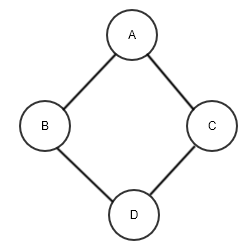
\includegraphics[scale=0.8]{pictures/undirected_graph.png}
    \caption{An example of an undirected graph}
    \label{graph}
\end{figure}
\par A simple power network can be represented as a graph $\mathcal{G}:=(\mathcal{V},\mathcal{E})$, where $\mathcal{V} \in \mathbb{N}$ is the set of \textit{vertices} or \textit{nodes} and $\mathcal{E} \subseteq (\mathcal{V} \times \mathcal{V})$ the set of \textit{edges} \cite{graph_theory}. The nodes are connected via the edges and we consider the connection as \textit{undirected}. In graph theory, a node is considered \textit{incident} to an edge if the node is one of the two node the edge connects. An example of an undirected graph is shown in \ref{graph} \cite{un_graph}. 
\\As described in Definition \ref{prosumer_def}, a node from a power network in the form of a graph is a representation of a prosumer, so either a producer, consumer or idle. An edge represents the power lines that connects the prosumers to each other. Current flows through the power lines, feeding or drawing electricity to or from the nodes. This means that the current flows in both direction, which is why the graph is also considered as \textit{undirected}. 
\\ Let $N \in \mathbb{N}$ be the number of prosumers in a DC microgrid connected to each other. The prosumers are at grid nodes $j,k \in \{1,2,..,N\} =: \mathcal{N} \subset \mathbb{N}$. Then the number of the edges or \textit{number of power lines} is defined as \cite{lia_master}: 
\begin{align*}
    m &\leq \frac{N(N-1)}{2}
\end{align*}
The index $h \in \{1,2,..,m\} =: \mathcal{M} \subset \mathbb{N}$ is then used for the power lines \cite{lia_master}. The connection $jk$ is incident with the grid nodes $j$ and $k$ and starts from node $j$ to node $k$. It contains the power line $h$. \\To describe the relationship between between nodes and power, we use the \textit{incidence matrix} $\boldsymbol{M}$ of a network graph with the dimension $m \times N$ with 
\begin{align}
\label{equation:incidence_def}
    \boldsymbol{M} &= \begin{bmatrix} m_{1,1} & \dots & m_{1,N} \\ \vdots & \ddots& \vdots \\ m_{m,1} & \dots & m_{m,N} \end{bmatrix} \in \mathbb{R}^{m \times N}
\end{align}
where the entries for each connection are $m_{h,j} = 1$ and $m_{h,k} = -1$. All other entries $m_{h,\kappa}=0$ are the non-incident nodes $\kappa \in \mathcal{N}$ to the power line h \cite{lia_master}. \\ With the incidence matrix $\boldsymbol{M}$, the network topology is uniquely described. By using the incidence matrix, we can describe the Kirchhoff Laws in the network as constraints \cite{lia_master}. Since the topic of this thesis is to control the overall model of the prosumer-based direct current microgrid with the iterative learning control method, the next section introduces the two-layer control with the iterative learning control method.
\section{The two-layer control with the iterative learning control method}
\label{sec:ilc}
In this section, we get to know the basics of the two-layer control with the \textit{iterative learning control method}, by introducing in \ref{subsec:feedback} the \textit{standard control feedback loop}, which is the base for many control applications. We will later delve into the \textit{low-layer-control} and the \textit{high-layer-control}, that result the \textit{two-layer-control method} (\ref{subsec:twolayer}), one specialization of which is the iterative learning control (\ref{subsec:ilc}).
%Seite 170 - Iterative Learning control 
\subsection{Basics of of the standard control feedback loop}
\label{subsec:feedback}
\begin{figure}[h]
\centering
    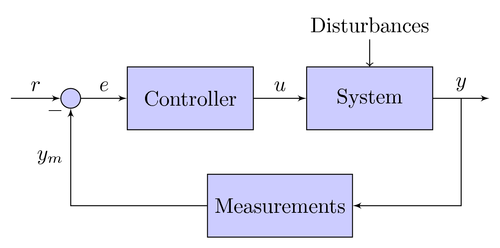
\includegraphics[scale=0.5]{pictures/control-system-principles.png}
    \caption{Closed-loop model in standard feedback control loop block representation \cite{cs_princi}, with the definitions as in \cite{cs_princi_wiki,lia_master} $r$ for the reference, $e$ for the measured error, $u$ for the system input, $y$ for the system output and $y_m$ for the measured system output}
    \label{clm_standard_feed}
\end{figure}
In engineering, processes in form of a dynamical (time-dependent) system need to be controlled, in order to achieve control stability and an optimal behavior. Therefore, a \textit{controller} is designed uniquely for the to-be-controlled system, to automatically regulate the output and keep it within the systems desired input value or “set point” \cite{oploop}. If the system input changes for whatever reason, the output of the system must respond accordingly and change itself to reflect the new input value \cite{oploop}. 
\\In most systems the controlling process, the controllers actions depend on the feedback from the process. In other words, we can control a process by adding an amount of the output to the measured error, so the actual output is compared with the desired and the error can be reduced or even eliminated. 
This type of control system is called \textit{closed-loop control system} or \textit{feedback control system} and two-layer controllers belong to this family of controls. \\The basics of the \textit{two-layer control method}, which is going to be used in this research, are going to be explained in the next section \ref{subsec:twolayer}.
\subsection{Two-layer control}
\label{subsec:twolayer}
Microgrids control and management are, not as in the standard feedback control loop described in section \ref{subsec:feedback}, usually divided in multiobject tasks, covering mostly different time scales and physical levels \cite{controldc}. This schema is divided hierarchically and every layer has a different task from e.g. frequency control to energy management. Two-layer architectures, which are used in our research as control architecture are e.g. used among others for economic optimization \cite{hier_control}.\\
As described in \cite{paperilc}, in microgrids, hierarchical control is
typically divided in \textit{primary}, \textit{secondary} and \textit{tertiary control}, also called energy management, referring to the same
tasks. In particular it is said that "[...] \textit{primary control is responsible for fast frequency
stabilization and reacts in seconds, secondary control restores the frequency to its setpoint in terms of minutes
and tertiary control refers to economic dispatch questions
in the time scale of hours and days[...]}" \cite{paperilc}. The definition is referring to systems, where frequency is a control property. Since in direct current microgrids no frequency appears, primary, secondary and tertiary control, proposed by Meng and Ferrai Trecate in \cite{controldc} and Luis Orlando Polanco Vasquez et al. in \cite{controldc_energy_man} are considered as follows: 
\begin{enumerate}
    \item \textit{Primary control} performs the control of local power,
    voltage, and current. It normally follows the set-points
    given by upper level controllers and is communication-less power sharing among DERs \cite{controldc}. 
    \item \textit{Secondary control} appears on top of primary control.
    It deals with issues in the system level, such as power quality regulation, microgrid synchronization with external grid for smooth reconnection [...] and so on \cite{controldc}.
    \item \textit{Tertiary control} is issued with optimization, management, and overall system regulations \cite{controldc}. It considers the economical concerns [...] and manages the power flow between the microgrid and the main grid \cite{controldc_energy_man}.
\end{enumerate}
In decentralized hierarchical control, regulation takes place with only local information \cite{controldc_energy_man} and the control functions can be distributed into local controllers, or in our case \textit{lower-layer controllers} and upper-level or \textit{higher-layer controllers}. Primary and secondary control can be combined as the lower-layer control and tertiary control as the higher-layer control. The grid itself and the low-level controller form the \textit{compound plant} Placing the higher-layer controller into the system can save lower-layer control energy \cite{paperilc}. \\ In this research, the two-layer schema is used with an \textit{iterative learning controller} as a higher-layer controller, proposed by Strenge et al. in \cite{paperilc}. The iterative learning method is going to be introduced in the next section.
\subsection{Iterative learning control}
\label{subsec:ilc}
\begin{figure}[h]
	\centering
	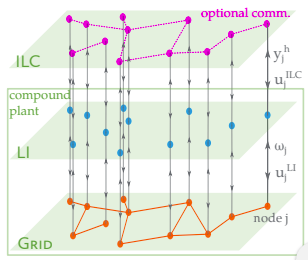
\includegraphics[scale=0.7]{pictures/control_hierarchy.png}
	\caption{Control hierarchy with low-level control (LI) and iterative learning controller (ILC) \cite{paperilc}. Here, the grid current is alternating and the control achievement is the bounded frequency deviation ($\omega_j$)}
	\label{fig:control_hier}
\end{figure}
The \textit{iterative learning control} (ILC) is a method that addresses the problem of transient response performance for systems that operate in a repetitive mode \cite{vl_ilc}. Based on the errors observed during past operations, the transient response is improved by adjusting the input to the plant during future \cite{vl_ilc}.
\begin{figure}[h]
\centering
    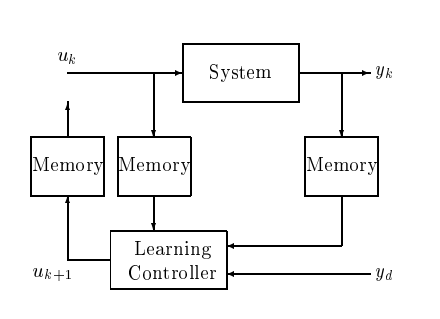
\includegraphics[scale=0.56]{pictures/ILC_schema.png}
    \caption{Iterative learning control configuration}
    \label{fig:figure_ILC}
\end{figure}
The basic idea of iterative learning control is illustrated in Figure \ref{fig:figure_ILC} \cite[p.427]{moore_ilc}. The ILC algorithm has the form, proposed by \cite{paperilc}
\begin{align}
    u^{c+1}= u^{c}- Ly^{c}
\end{align}
The power $c$ is the cycle number. In this work $c$ has the duration of one day. During the $c$-th repetition $u^c$ is inputted, producing an output $y^c$. While the input and output is memorized, this output is observed as an error and based on this the next input $u^{c+1}$ is modified. The new input is designed so that the new error is smaller than the previous input. By time shifting we get
\begin{align}
    u^{c}= u^{c-1}- Ly^{c-1} \label{eq:ilc_inp_th}
\end{align}
with $L$ a single scalar parameter $ L = \kappa \in \mathbb{R}_{>0}$.\\
The proposed ILC approach is applied to learn a power infeed that compensates the periodic demand component and to save lower-layer-energy \cite{paperilc}. \\Now that the basics of prosumer-based direct current microgrids and the iterative learning control have been introduced, in the next chapter the network dynamics with the lower-layer and higher-layer controller can be modeled.
